\documentclass[]{scrartcl}
\usepackage[spanish]{babel}

\decimalpoint
%opening
\usepackage{xcolor}
\usepackage{mathtools}
\usepackage{graphicx}
\usepackage{enumitem}
\usepackage{hyperref}
\newcommand{\tt}[1]{\texttt{#1}}

\newcommand{\that}[0]{\texttt{THAT~}}

\usepackage{siunitx}
\sisetup{output-decimal-marker = {.}}


\hypersetup{
	colorlinks=true,       % Activa el color en los enlaces
	linkcolor=blue,        % Color para enlaces internos
	filecolor=blue,        % Color para archivos locales
	urlcolor=blue,         % Color para URLs externas
	pdfborderstyle={S} % Añade un subrayado a nivel de PDF (opcional)
}

\title{Práctica 2: estabilidad de sistemas realimentados}
\author{Leonardo Bermeo}

\begin{document}
	
	\maketitle



\section{Generador de onda cuadrada\label{sec:cuadrada}}
El computador analógico \tt{THAT} tiene una señal que indica cuando los integradores de cómputo son \emph{reseteados} periodicamente al elegir uno de los modos repetitivos (\tt{REP} o \tt{REPF}). Dicha señal está en la salida \tt{TR}. Vamos a usar esa señal para generar una onda cuadrada que nos permita obtener la respuesta al escalón para los sistemas analógicos que implementaremos.
\begin{enumerate}[label=\alph*)]
	\item Conecte el cable RCA blanco a las señales \texttt{TR} (trigger) y \texttt{U} del \tt{THAT} como se muestra en la figura~\ref{fig:jackrca}. 
%
\begin{figure}[h!]
	\centering
	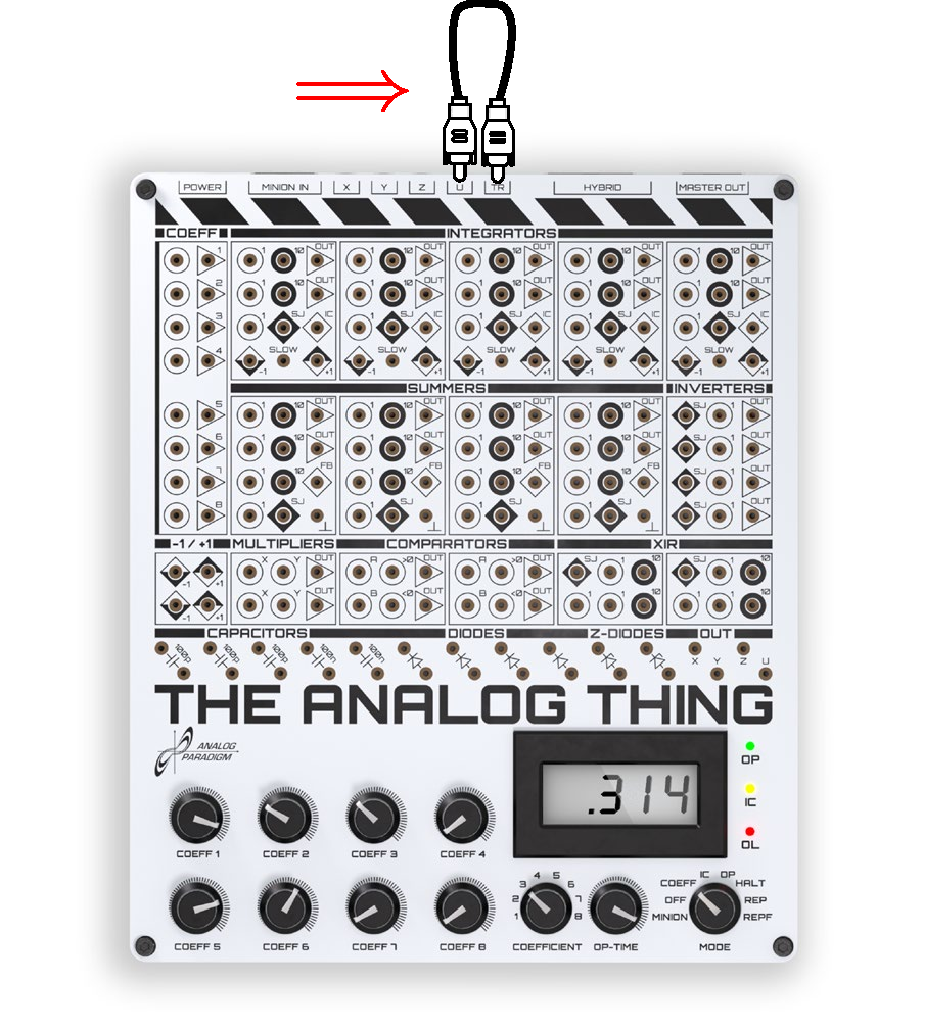
\includegraphics[width=0.5\linewidth]{figuras/jackrca}
	\caption{Conector RCA}
	\label{fig:jackrca}
\end{figure}
\newpage
\item  Realice cuidadodamente las conexiones que se ilustran en la figura \ref{fig:onda_cuad}
%
\begin{figure}[h!]
	\centering
	
\includegraphics[width=0.8\linewidth]{figuras/onda_cuadrada1}
	\caption{Conexiones para la onda cuadrada}
	\label{fig:onda_cuad}
\end{figure}
%\item Conecte los cables RCA desde las señales \texttt{X} e \texttt{Y} del \tt{THAT} a los canales 1 y 2 del osciloscopio como se muestra, usando los conversores de RCA a BNC suministrados. 
%%
%\begin{figure}[h!]
%	\centering
%	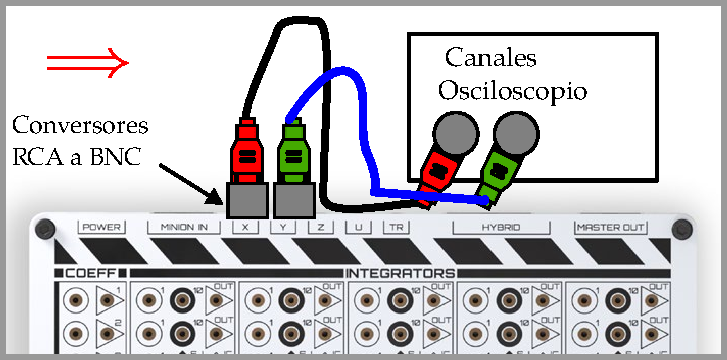
\includegraphics[width=0.7\linewidth]{figuras/canales_osc}
%	\caption{Conexiones para el osciloscopio}
%	\label{fig:canales_osc}
%\end{figure}

\item Conecte el cargador USB-C a la entrada \texttt{POWER} del \tt{THAT}.

\item Ajuste el selector  \texttt{MODE} en \texttt{REPF}  (repetitive fast),  es decir, con repetición rápida del reset de los integradores . Ajuste el tiempo entre cada reset de los integradores con el potenciométro de \texttt{OP-TIME} al máximo, como se ilustra en la figura~\ref{fig:botones}.  
%
\begin{figure}[h!]
	\centering
	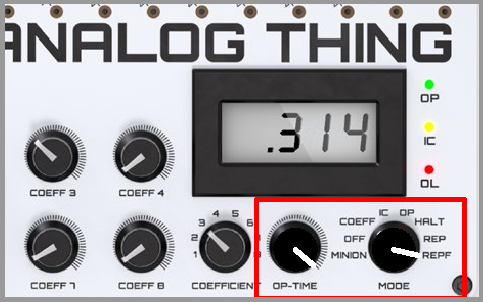
\includegraphics[width=0.5\linewidth]{figuras/botones_repf}
	\caption{Ajuste de los botones}
	\label{fig:botones}
\end{figure}


\item Sincronice adecuadamente con el menu de trigger el canal 1 del osciloscopio. Debe estar visualizando una señal cuadrada como la mostrada en la figura~\ref{fig:senal_osc}. El osciloscopio debe estar en acople CC en toda esta práctica.
%
\begin{figure}[h!]
	\centering
	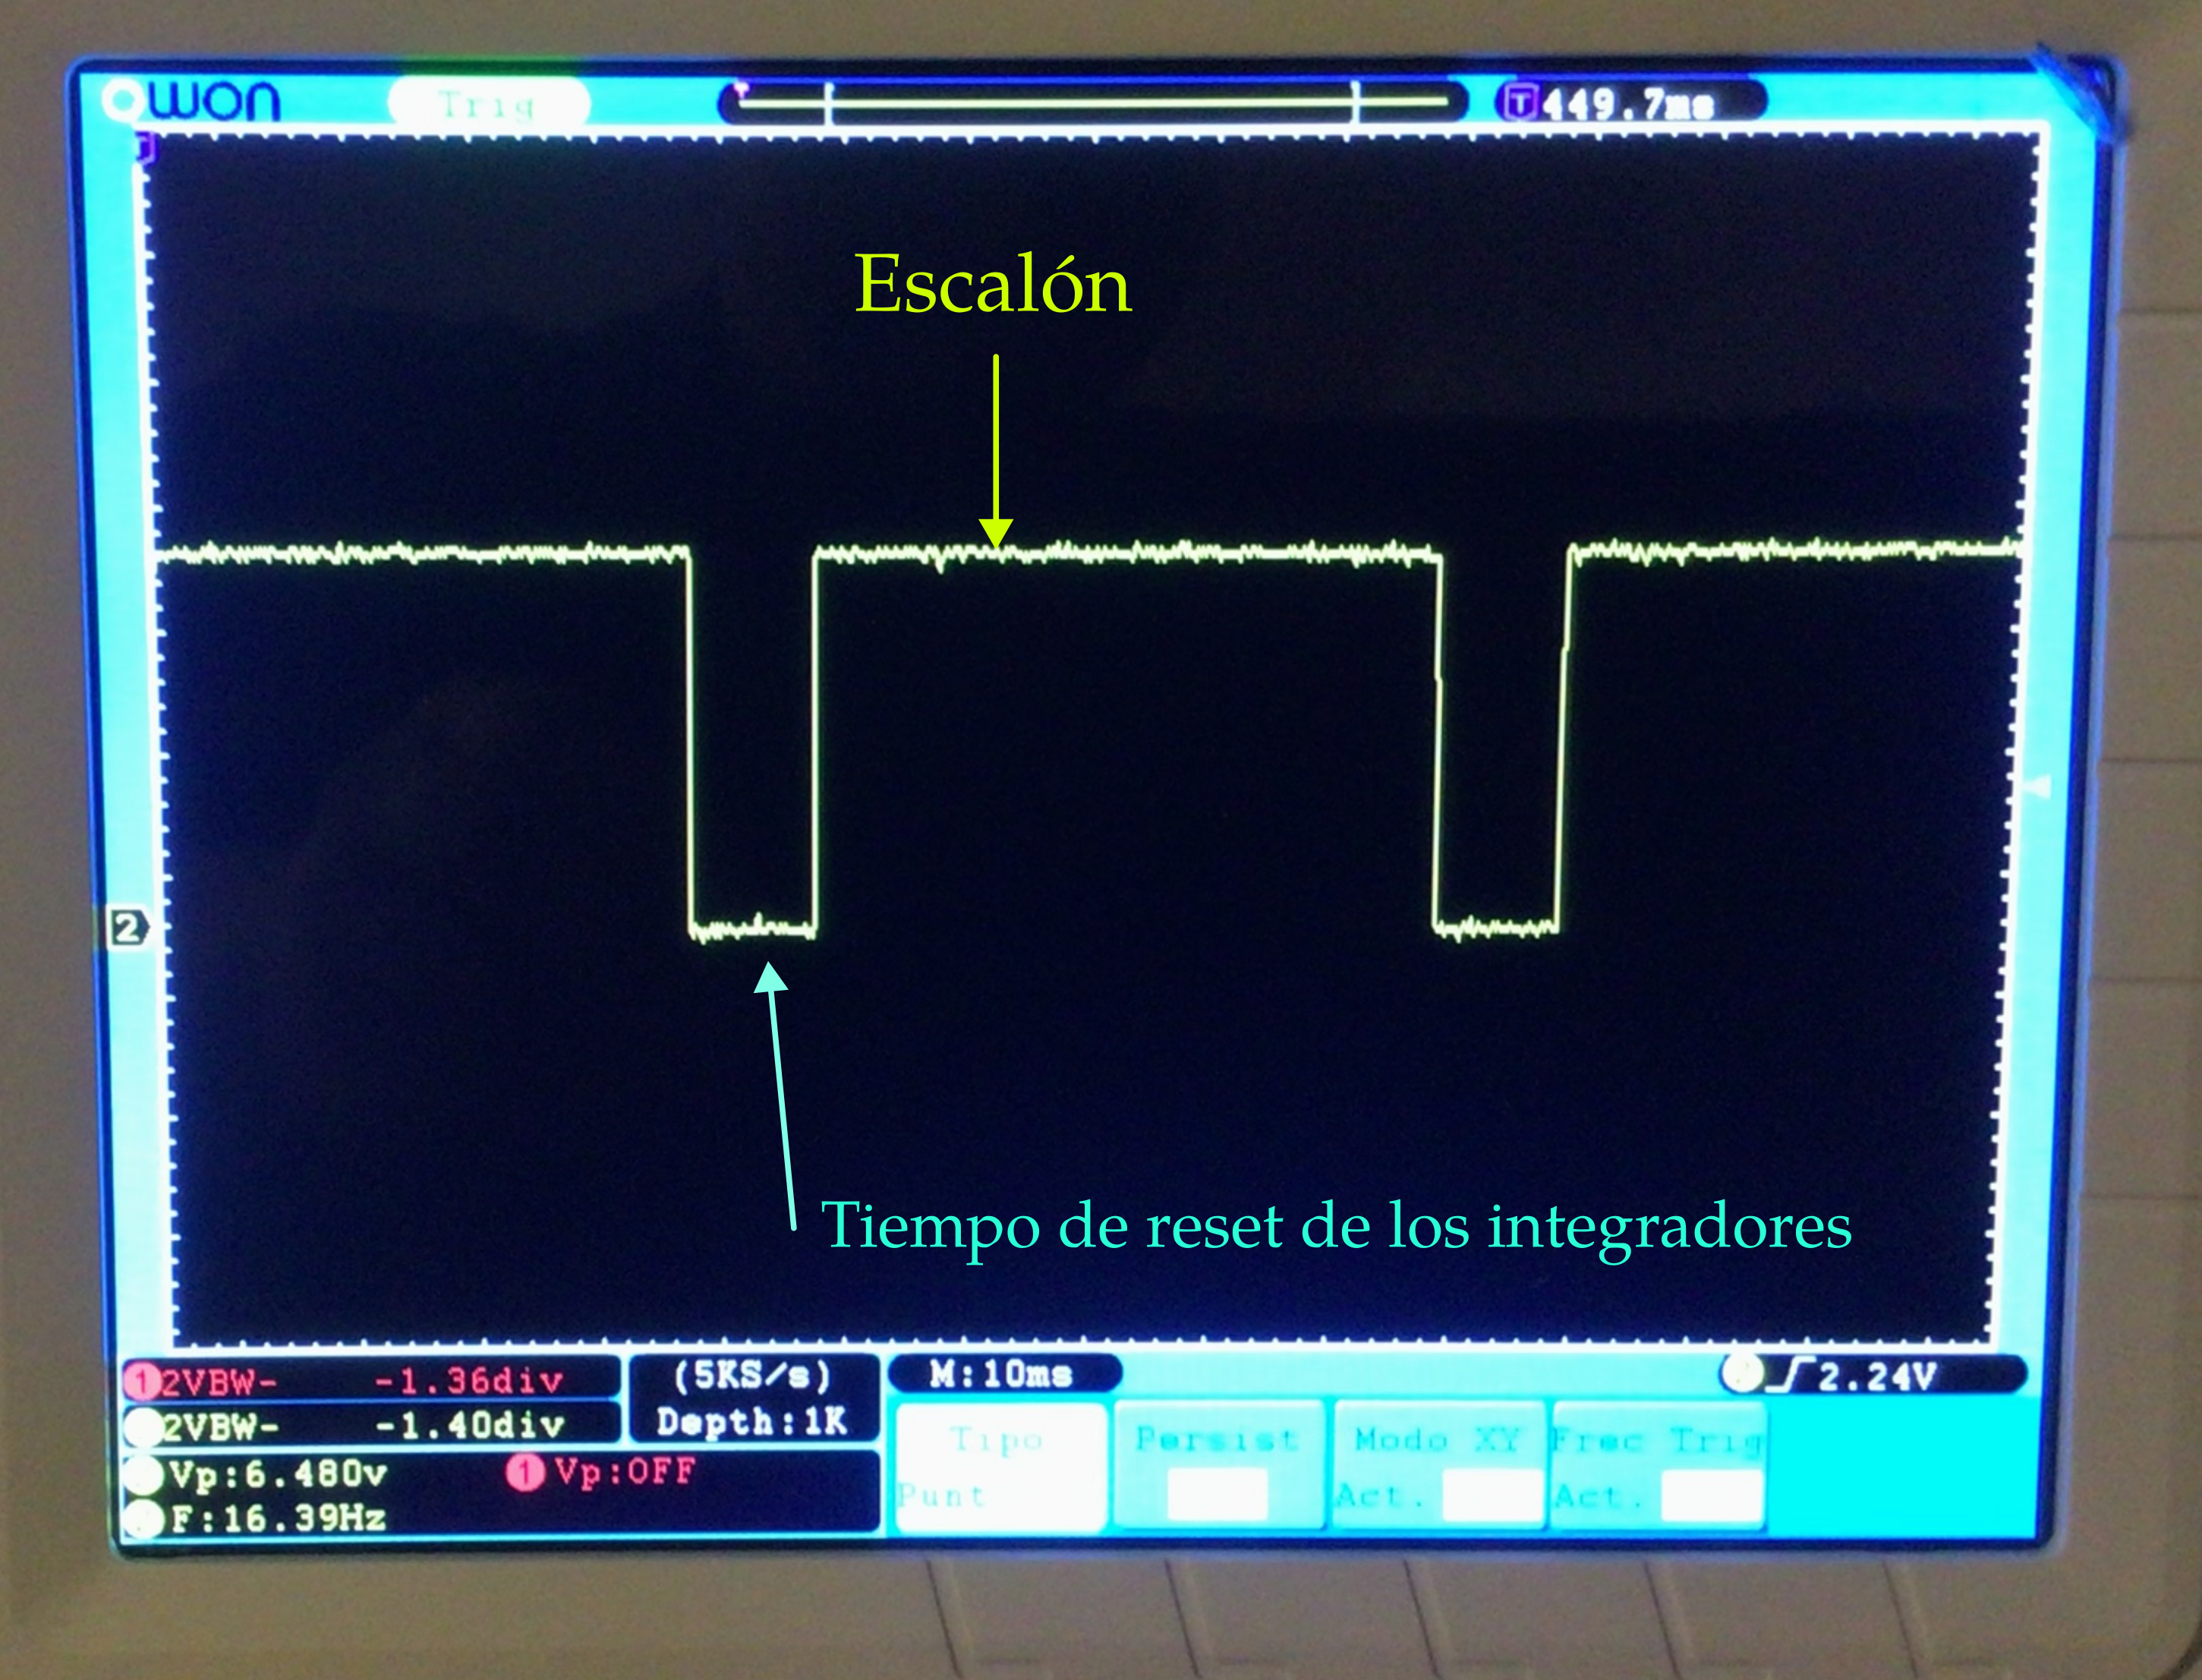
\includegraphics[width=0.6\linewidth]{figuras/osc_cuadrada1}
	\caption{Señal cuadrada}
	\label{fig:senal_osc}
\end{figure}
\newpage
\item Verifique que el potenciómetro \tt{COEFF 8}  ajusta la amplitud del escalón la onda cuadrada. Ajuste la amplitud en 1V,  aproximadamente. 
 %
 \begin{figure}[h!]
 	\centering
 	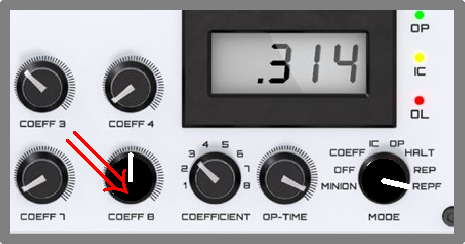
\includegraphics[width=0.5\linewidth]{figuras/amplitude_cuadrada}
 	\caption{Botón de control de Amplitud}
 	\label{fig:boton_amplitud}
 \end{figure}

\end{enumerate}

\section{Estabilidad de un sistema de tercer orden con control proporcional}

En esta  sección vamos a analizar la estabilidad del sistema realimentado de la figura~\ref{fig:realimentado}:
%
\begin{figure}[h!]
	\centering
	
\includegraphics[width=.65\textwidth]{figuras/realimentado}
	\caption{Sistema realimentado}
	\label{fig:realimentado}
\end{figure}

Este sistema tiene función de transferencia de lazo cerrado $T(s)$, dada por:
\begin{align}
T(s) = \dfrac{Y(s)}{R(s)} &= \dfrac{kG(s)}{1+kG(s)}\nonumber\\
	   &= \dfrac{k}{s^3+1.5s^2+0.5s+k}
	   \label{equ:realimentado}
\end{align}



Queremos analizar experimentalmente la estabilidad de $T(s)$  para variaciones del parámetro $k$ en que $0 \leq k \leq 1$, usando el \that


\subsection{Implementación}

Note que la función $G(s)$ en el lazo realimentado la podemos expresar como:

\begin{align}
	G(s)&=G_1(s) \times G_2(s) \times G_3(s) \nonumber\\
	&=\dfrac{1}{s} \times \dfrac{1}{s+0.5} \times \dfrac{1}{s+1}.
\end{align}

 Y cada bloque de primer orden lo podemos realizar como se ilustra en la figura~\ref{fig:analoghurwitz}
 %
\begin{figure}[h!]
	\centering
	
\includegraphics[width=.9\textwidth]{figuras/analoghurwitz}
	\caption{Implementación de computador analógico.}
	\label{fig:analoghurwitz}
\end{figure}


\subsection{Pasos de implementación}

\begin{enumerate}[label=\alph*)]

	
	
	\item Implemente cuidadosamente en el \that~ el diagrama de la figura \ref{fig:analoghurwitz}. Use los bloques apropiados.
	\item Conecte el canal 1 y el canal 2 a la entrada $R$ y la salida $Y$, del sistema realimentado, respectivamente. 
	
	\item Ponga el \tt{THAT} en modo \tt{REPF}.
	
	\item Varie el coeficiente correspondiente a $k$ y determine por la respuesta percibida en el osciloscopio, el punto en que el sistema cambia de estable a inestable. Registre este valor pasando el \tt{THAT} al modo \tt{COEFF}. Compare con lo obtenido mediante el test de estabilidad de Routh Hurwitz. 
	
	\item Encuentre experimentalmente un valor de $k$ que en su concepto produce un desempeño satisfactorio de control. Calcule la localización de los polos de lazo cerrado para este caso. Muestre la respuesta experimental obtenida en este caso y haga un dibujo de los polos en el plano complejo.
	
	\item Calcule los polos del sistema de lazo cerrado para un valor de $k$ en que el sistema es inestable. Muestre la respuesta experimental obtenida en este caso y haga un dibujo de los polos en el plano complejo.
	
	
\end{enumerate}

\section{Estabilidad de un sistema de tercer orden con control PI}
Consideremos el sistema con control PI mostrado en la figura~\ref{fig:controlpi}.

\begin{figure}[h!]
	\centering
	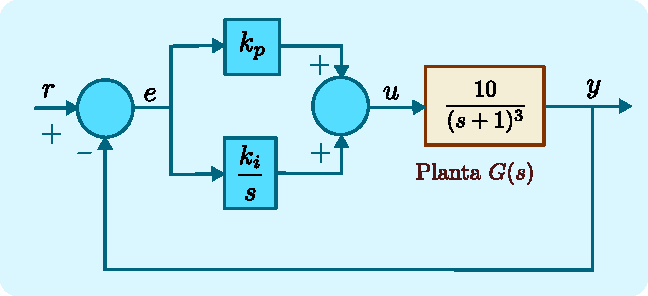
\includegraphics[width=.8\textwidth]{figuras/controlPI}
	\caption{Implementación de computador analógico.}
	\label{fig:controlpi}
\end{figure}

Realice lo siguiente:

\begin{enumerate}[label=\alph*)]
	
	\item Diseñe un dibujo de computación analógica  que permita implementar el sistema con control PI de la figura~\ref{fig:controlpi} con el \that.
	
	\item Implemente cuidadosamente su diseño, use el mismo montaje de generación de onda cuadrada para la referencia $R$, montado anteriormente.
	
	\item Ajuste un valor de $k_i$ por ejemplo $k_i=0.2$, y verifique experimentalmemnte el rango de valores de $k_p$ en que el sistema permanece estable. Compare con la región de estabilidad teórica.
	
	\item Ajuste un valor de $k_p$, por ejemplo $k_p=0.35$, y verifique experimentalmemnte el rango de valores de $k_i$ en que el sistema permanece estable. Compare con la región de estabilidad teórica.
	
	\item Observe el gráfico de la región de estabilidad teórica y con base en ella, ajuste experimentalmente unos valores de $k_p$ y $k_i$ que logren un control bien satisfactorio. Pruebe ampliamente variando los coeficientes de $k_p$ y $k_i$ y reporte los mejores valores encontrados. Grafique el punto $(k_p, k_i)$ encontrado experimentalmente en la  región de estabilidad.
	
\end{enumerate}


\end{document}
